\chapter{Experimental Setup}
%%ATLAS is a multipurpose detector positioned around one of the 4 primry interaction points of the Large Hadron Collider (LHC) in Geneva, Switzerland. The LHC collides protons at a center of mass energy of 13 TeV, for Run 2, at a rate of approximately 600MHz. 
\section{Hadronic Colliders}
Hadron colliders use two beams of hadrons, particles made of three quarks, typically proton-proton or proton-antiproton. The large mass of the hadrons results in smaller synchrotron radiation in circular accelerators, when compared to leptonic colliders with equivalent energies, as the radiated power scales as ${\frac{1}{m^{4}}}$. This allows hadronic colliders to reach much larger center of mass energies with the same size circular ring. \newline

\indent While hadronic colliders typically have larger collision energies, they also have significantly ``messier" collisions. In leptonic colliders, the only final state particles come from the colliding particles. In hadronic colliders, not all of the constituent partons of the hadrons interact in the hard collision. This means the exact collision energy is not known. Each parton only carries a portion of the hadron momentum, making it impossible to know the longitudinal center of mass. 



\section{The Large Hadron Collider}
%Source http://iopscience.iop.org/article/10.1088/1748-0221/3/08/S08001/meta
%Source  http://cds.cern.ch/record/2119882
%Source PSB: http://accelconf.web.cern.ch/Accelconf/p69/PDF/PAC1969_0959.PDF
% PS https://cds.cern.ch/record/1479637/files/1959_E_p29.pdf
% file:///C:/Users/jmyers/Documents/2018/Thesis/Sources/1102.1949.pdf
% https://cds.cern.ch/record/941318/files/p361.pdf
The Large Hadron Collider (LHC) is a 27 kilometer ring underneath the Franco-Swiss border. The LHC accelerates beams of protons (or ions) to a center of mass energy of up to 13 TeV(5 TeV) in two antiparallel beams around the ring. The particles are then collided at 4 primary interaction points each of which has a dedicated detector: ATLAS, CMS, ALICE, and LHCb.\linebreak
\indent In order to get the protons up to the collision energy, the LHC uses a series of smaller accelerators in the injection chain. The start of the chain, and the source of protons for the LHC, is the Linear Accelerator 2 (Linac 2) \cite{accelerator:1997427}. Hydrogen gas is taken from a bottle and the electrons are stripped off by an electric field. When only the protons remain, they pass through radiofrequency (RF) cavities. These RF cavities are shaped, such that the electromagnetic waves are resonant inside of the cavity and build up energy. When charged particles pass through the cavity, they feel the force of the electric field and are pushed forward. The field in the RF cavities oscillates at a frequency specific to the distance from the previous cavity, giving a specific energy to a passing particle depending on the momentum. When a particle arrives early to the cavity, the field removes some of the energy from the particle, when it arrives late it gets a boost from the cavity to get it back to the target energy. When a proton reaches the end of Linac 2, it has an energy of 50 GeV.\linebreak

\begin{figure}[h]
\begin{center}
\includegraphics*[width=0.70\textwidth] {figures/CERN_Accelerator_Complex}%Taken from https://cds.cern.ch/record/2119882
\caption[CERN accelerator complex \cite{DeMelis:2119882}]{CERN accelerator complex \cite{DeMelis:2119882}}
\label{fig:CERN_ACC}
\end{center}
\end{figure}


\indent After the protons leave the Linac 2, they enter the Proton Synchrotron Booster (PSB)\cite{Reich}. The PSB accelerates the protons to an energy of 1.4 GeV and are passed to the Proton Synchrotron (PS) in two batches, 1.2 seconds apart. The PS accelerates protons to 26 GeV and delivers them to the next step in the injection chain, the Super Proton Synchrotron (SPS) in a series of 4 batches, 3.6 seconds apart. The SPS is the second largest accelerator at CERN. As protons pass through, they as boosted to an energy of 450 GeV \cite{Brianti:340514}. Once the particles reach this energy, they are split and injected into the LHC in two opposite directions. Once in the LHC, the protons are brought up to their target energy of 6.5 TeV per beam.
\subsection{LHC Magnets} 
Accelerators depend on powerful magnets to bend and focus the colliding particles. The LHC is the most powerful particle accelerator that has ever existed. In order to make this possible, the LHC was constructed with the most advanced magnet technology available at the time. These magnets are cooled to below 2 K and produce a field to over 8 T.\linebreak
\begin{figure}[h]
\begin{center}
\includegraphics*[width=0.60\textwidth] {figures/Cross-section-of-a-LHC-superconducting-cryodipole-85}%Taken from http://cds.cern.ch/record/1129806/
\caption[Cross-section of cryodipole (lengths in mm)]{Cross-section of cryodipole (lengths in mm)}
\label{fig:cryo_cross}
\end{center}
\end{figure}

\indent The LHC uses 1104 superconducting, dipole magnets to bend the beam of particles around the ring, and another 128 in the beam dump.  Each dipole is 15 m long and weigh 35 tonnes. A current of 11,000 Amps pass through an octant in series to produce the magnetic field. Each octant is powered independently. A cross section of a dipole can be seen in Figure ~\ref{fig:cryo_cross}. Inside of these dipoles, there are sextupole, octopole and decapole magnets to correct for small imperfections in the magnetic field at the outside of the dipole \cite{Evans_2008}. A key feature of the dipole magnets i the 2-in-1 configuration. Where each dipole generates a magnetic field in the opposite direction in the two pipes, figure ~\ref{Fig:bfield}. Allowing a single dipole to bend the two beams in opposite directions.  \linebreak

\begin{figure}[h]
\begin{center}
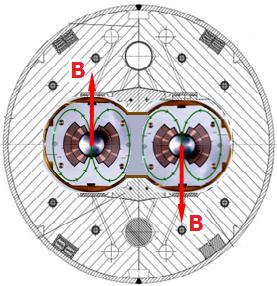
\includegraphics[scale=0.65]{figures/dipole_bfield}
\caption{Magnetic field configuration of the dipole magnets \cite{Lorentz}}
\label{Fig:bfield}
\end{center}
\end{figure}

\indent	It is also important to focus the beam to a small area, in order to maximize the collisions. This is achieved by 
pair of quadrupole magnets. One magnet focuses in the horizontal plane, defocusing in the vertical, and the other focuses in the vertical plane, defocusing in the horizontal. These magnets work together to focus the beam in both planes. 
\subsection{Luminosity and Pileup}
In a collider, a key statistic is the rate of events produced. This value is called luminosity (${\mathcal{L}}$) and is defined by equation ~\ref{eq:part_lumi} \cite{Aaboud:2016hhf}, where ${\sigma}$ is the cross section, or probability of collision.
\begin{equation}
\label{eq:part_lumi}
\mathcal{L} = \frac{1}{\sigma}\frac{dN}{dt}
\end{equation}
%L = 1/sigma dN/dt
In order to maximize this number, the LHC collides bunches of protons. These bunches are made up of ${1.15\times10^{11}}$ protons. In the LHC during run 2, the LHC beams had around 2500 bunches organized into a train of bunches, separated by small gaps with a larger gap at the end of the train. The luminosity per proton pair crossing, equation ~\ref{eq:lumipp}
\begin{equation}
\label{eq:lumipp}
\mathcal{L} = \frac{1}{4\pi\sigma_{x}\sigma_{y}}
\end{equation}
is then multiplied by the number of protons per bunch for the two beams, ${N_{1}}$ and ${N_{2}}$, and by the number of bunches ${N_{b}}$ and the frequency \textit{f}. The use of bunches changes the luminosity calculation to equation ~\ref{eq:full_lumi})
\linebreak
\begin{equation}
%source (https://cds.cern.ch/record/941318/files/p361.pdf eq 16)
\label{eq:full_lumi}
\mathcal{L} = \frac{N_{1}N_{2}fN_{b}}{4\pi\sigma_{x}\sigma_{y}}
\end{equation}

\indent By integrating the luminosity over the running time of the LHC, you obtain the total delivered luminosity, Fig ~\ref{fig:lumi}. By multiplying the integrated luminosity by the probably of a particular final state, or the cross section, it is possible to obtain the number of times a final state is produced.\linebreak

\begin{figure}[H]
\begin{center}
\includegraphics*[width=0.60\textwidth] {figures/intlumivstimeRun2}%Taken from https://twiki.cern.ch/twiki/bin/view/AtlasPublic/LuminosityPublicResultsRun2
\caption[Integrated Lumi]{Cumulative luminosity versus time delivered to ATLAS (green) and recorded by ATLAS (yellow) during stable beams for pp collisions at 13 TeV centre-of-mass energy in LHC Run 2.  (figure from the ATLAS Collaboration)}
\label{fig:lumi}
\end{center}
\end{figure}

\subsection{Pileup}
\indent By interacting bunches of protons at a time, it is possible for more that one pair of protons to undergo an inelastic collision. In fact, during Run 2,  the average number of interactions per bunch crossing, or pileup, was roughly 32. The profile of the pileup for all of Run 2 can be seen in Figure ~\ref{fig:mu} 

\begin{figure}[H]
\begin{center}
\includegraphics*[width=0.60\textwidth] {figures/mu_2015_2018}%Taken from https://twiki.cern.ch/twiki/bin/view/AtlasPublic/LuminosityPublicResultsRun2
\caption[Number of interactions per bunch crossing]{Shown is the luminosity-weighted distribution of the mean number of interactions per crossing for the 2015-2018 pp collision data at 13 TeV centre-of-mass energy. All data recorded by ATLAS during stable beams is shown, and the integrated luminosity and the mean mu value are given in the figure. (figure from the ATLAS Collaboration)}
\label{fig:mu}
\end{center}
\end{figure}

\subsection{Detector Coordinates}
%Source
Within the ATLAS detector, the interaction point defines the origin of the coordinate system. The z-axis, the longitudinal axis, runs along the beam line, the positive x-axis points toward the center of the LHC ring, and the positive y-axis points toward the surface. The detector is also described in r, ${\eta}$, ${\phi}$ coordinates. With the transverse plane, the plane perpendicular to the beam line, being described by r and ${\phi}$. The radial coordinate, r, describes the distance from the beam line. The azimuthal angle, ${\phi}$, is the angle from the x-axis around the beam line. The final coordinate, ${\eta}$, is referred to pseudorapidity and is defined as ${\eta = -\ln(\tan(\frac{\theta}{2}))}$. With ${\theta}$ being the angle from the y-axis. Differences in ${\eta}$ are Lorentz invariant under longitudinal boosts. Meaning difference in the rest frame of colliding particles are not important for massless particles. In ATLAS, the large particle boost allows for all particles to be considered massless when considering ${\eta}$. Additionally, particle are produced uniformly in ${eta}$. For these reasons, ${\eta}$ is preferred over ${\theta}$. A pictoral representation can be seen in Figure ~\ref{fig:coord}. The variable ${\Delta{R}=\sqrt{\eta^{2} + \phi^{2}}}$ is often used to describe the distance between detector objects.

\begin{figure}[h]
\begin{center}
\includegraphics*[width=0.60\textwidth] {figures/coordinate}
\caption[Detector coordinate system]{Detector coordinate system \cite{phdthesis}}
\label{fig:coord}
\end{center}
\end{figure}



\section{Detector Overview}
%Source
\begin{figure}[h]
\begin{center}
\includegraphics*[width=0.60\textwidth] {figures/ATLAS_det}
\caption[The ATLAS detector]{The ATLAS detector \cite{Collaboration_2008}}
\label{fig:ATLAS_det}
\end{center}
\end{figure}
The ATLAS detector, Figure~\ref{fig:ATLAS_det}, is a general purpose detector and the largest on the LHC.  It is made up of concentric subsystems, each with a specialized task: the inner detector, which is responsible for measuring the charge and momentum of charged particles; the calorimeters, which are responsible for measuring the energy of different electromagnetic and hadronic particles; the muon spectrometer, which measures the momentum of minimum ionizing particles (MIP), like muons; and the magnet system, which is responsible for bending the charged particles in the detector, allowing their charge and momentum to be measured. The subdetectors feed into a vast Trigger and Data Acquisition (TDAQ) system that is responsible for selecting collision events with interesting characteristics and reading out detector elements.
%
\subsection{The Inner Detector}
%Source Inner detector TDR, I: https://cds.cern.ch/record/331063?ln=en
%Source Inner detector TDR, II: https://cds.cern.ch/record/331064?ln=en
%Source IBL TDR: https://cds.cern.ch/record/1291633?ln=en
\begin{figure}[h]
\begin{center}
\includegraphics*[width=0.60\textwidth] {figures/inner_3D}%Taken from ID TDR
\caption[Cross section of the Inner Detector.]{Cross section of the Inner Detector.}
\label{fig:ID_cs}
\end{center}
\end{figure}
%Tile: https://cds.cern.ch/record/2004868/files/ATL-TILECAL-PROC-2015-002.pdf
%Tile TDR: https://cds.cern.ch/record/331062?ln=en
%LAr TDR: https://cds.cern.ch/record/331061?ln=en
%LAr: https://www.physics.utoronto.ca/~krieger/procs/Krieger_NSS05_Proc.pdf
%
%Got To Here
%
The inner detector (ID), Figure~\ref{fig:ID_cs}, is the closest system to the beam pipe and is made of 4 separate pieces. In order of distance from the beam pipe: The Insertable B-Layer (IBL) \cite{Capeans:1291633}, the Pixel Detectors, the Semiconductor Tracker (SCT), and the Transition Radiation Tracker (TRT) \cite{CERN-LHCC-97-016}. These subsystems work together to give charged particle tracking within the pseudorapidity range of ${|\eta| < 2.5}$. When a charged particle passes through the silicon semiconductor detector in the IBL, Pixel and SCT, an electron-hole pair is created in the silicon. These electron-hole pairs drift toward the charged readout electrons on the surface of the detector. This gives a "hit" in the detector. The inner detector is immersed by a 2 T solenoid magnet, section ~\ref{ssec:mag}. The magnetic field causes charged particles to curve as they pass through the ID, leaving hits along the way. These hits are connected together into ``tracks" that show the trajectory of the particle as it passes through. The radius of curvature and direction of the track gives the sign of the charge, positive or negative, along with a momentum measurement of the particle. The other task of the ID is vertexing, or determining if the transient particle came from the interaction point of a slightly displaced point. This is used to identify long lived particles, like bottom or charm quarks, which travel a small distance before decaying. This is discussed further in section ~\ref{ssec:btag}. \linebreak
\indent The IBL is the newest addition to the ID, being installed during the 2016 shutdown. It is placed directly outside the beam pipe in order to maintain good vertexing and b tagging in increased pileup environments. In order to facilitate the insertion of the IBL, the beam pipe inner radius was decreased by 4 mm (from 29 mm to 25 mm). The IBL utilizes planar sensors, similar to the Pixel Detector, and 3D sensors, allowing electrons to interact with the bulk of the sensor as opposed to just the surface, and functions as a fourth pixel layer of the Pixel Detector. The addition of the IBL significantly improves the vertexing of the ID

%\begin{table}[h]
%\centering
%\begin{tabular}{cccc}\hline
%b tagger & Without IBL & With IBL & Ratio\\
%\hline\hline
%IP3D & ${83\pm{}1.5}$ & ${147\pm{3.4}}$ & ${1.8}$\\
%\hline
%IP3D+SV1 & ${339\pm{}12}$ & ${655\pm{}32}$ & ${1.9}$ \\
%\hline 
%\end{tabular}
%\caption{Rejection of light jets in \ttbar events without pileup for b efficiency of 60\%}\label{tab:ibl}
%\end{table}


\indent The Pixel Detector is a network of high granularity, silicon pixels which measure the 2D position of passing charged particles. The silicon pixels are n-doped silicon wafers. A high voltage is applied to the wafer and when a charged particle passes through the silicon an electron hole pair is created. The electron drifts to the electrode and creates a signal that is read out by the electronics.  The Pixel detector central barrel is divided into 3 cylindrical layers, the innermost layer is the B-layer, followed by Layer 1 and Layer 2. Each is covered in ${50\mu{m}}$ x ${400\mu{m}}$ silicon pixels. In order to ensure complete coverage, an end cap module is placed on each side of the barrel. The end-caps consist of 4 wheels, each with an inner and outer ring of trapezoid shaped silicon detectors. \linebreak
\indent The SCT is made of a barrel detector and two end-cap detectors. The barrel SCT has 4 cylindrical layers made up square modules covered with silicon microstrip detectors. 
The end-cap SCT tracker is made of rings of SCT modules with either silicon or galium arsenide. These rings are arranged into 9 wheels on each side of the barrel. In total, the SCT contains ${61 m^{2}}$ of silicon detectors with 6.2 million readout channels.\linebreak
\indent Outside of the silicon detectors lies the TRT. The TRT is a straw detector comprised of 50,000, 4mm diameter straws in the barrel and 32,0000 radial straws in the end-caps. There are 42,0000 electronic channels, which give a spatial resolution of ${170\mu{m}}$ per straw. The straws are filled with various mixtures of xenon argon, carbon dioxide, tetrafluoromethane and nitrogen gas. When a charged particle passes through the radiator between the straws, made of polypropylene, they emmit transition radiation photons. These photons ionize the gas in the straws and the free electrons are attracted to the positively charged wire and produce a signal that is later amplified and read out. The xenon in the gas mixture allows for accurate particle identification from the transition radiation photon detection. Transition radiation is emitted when a particle moves between two materials with different dielectric constants and is proportional to the Lorentz factor of the particle \cite{DOLGOSHEIN1993434}. This gives a good discrimination between electrons and charged pions. This entire system is enclosed within a solenoid magnet to bend the charged particles inside the ID.\linebreak

\subsection{Calorimeters}\label{ssec:calo}
%NOTE:::: Add general calo info




Outside of the solenoid magnet lies the calorimetry system. The calorimeters are responsible for measuring the energy of both charged and neutral particles, with the exception of MIPs and non-interacting particles such as neutrinos. The calorimeters can be broken into two distinct pieces, the liquid Argon calorimeter (LAr)\cite{CERN-LHCC-96-041} and the tile calorimeter \cite{CERN-LHCC-96-042}. \linebreak
\indent The Liquid Argon (LAr) calorimeter is a sampling calorimeter that is used for electromagnetic calorimetry for the entire range of acceptance (${|\eta{}|<4.8}$). It is also used for hadronic calorimetry for higher pseudorapidity ${1.4<|\eta{}|<4.8}$. The central barrel of the calorimeter (${|\eta{}| < 1.4}$) is made up of 1024 lead-stainless-steel converters with copper-polyimde multilayer readout boards. The plates and readouts are arranged in an ``accordion-shaped" geometry. This allows for complete azimuthal coverage with no gaps, giving an electromagnetic energy resolution that is uniform in azimuth. In between the accordion layers, liquid argon is used as the active medium. The system is enclosed in a cryostat to maintain the temperature of the detector. The LAr barrel is divided radially into 4 sampling layers. The granularity of the layers can be found in Figure ~\ref{fig:LAr_gran}. The layer closest to the beamline is the Presampler. This layer sits inside of the cryostat and is responsible for  correcting for the energy loss in front of the calorimeter (the same is done in the endcap). Inside the cryostat, there are 3 additional layers. The thickness of the layers is often described in terms of radiation lengths ${\chi_{0}}$. Where a radiation length is the distance a electron travels before it loses approximately 1/2 of it's energy to photon emission.  The front layer has a thickness of ${4.3\chi_{0}}$, followed by the middle layer with a thickness of ${16\chi_{0}}$ and the back layer of thickness ${2\chi_{0}}$. The shower maximum is contained in the second layer of the calorimeter, resulting in the bulk of the energy being absorbed in that layer. The design of the calorimeter allows for an energy resolution for electrons of ${\sigma_{E}/E \sim 10\%/\sqrt{\frac{E}{GeV}} \bigoplus 0.7\%}$ \cite{Aad:2014nim}.\linebreak 

\begin{figure}[h]
\begin{center}
\includegraphics*[width=0.60\textwidth] {figures/figure1-2}%Taken from LAr TDR
\caption[Sketch of the accordion structure of the EM calorimeter]{Sketch of the accordion structure of the EM calorimeter}
\label{fig:LAr_gran}
\end{center}
\end{figure}

\indent Forward from the barrel, there are two electromagnetic endcap (EMEC) wheels with a similar accordion structure to the barrel. One covering ${1.4 < |\eta{}| < 2.5}$ and one from ${2.5 < |\eta{}| < 3.2}$ Outside of the EMEC is the Hadronic endcap (HEC). This is also a copper-LAr sampling calorimeter. It has a simpler parallel plate design. Finishing out the LAr calorimeter is the Forward Calorimeter (FCal), which is contained in the endcap cryostat. This calorimeter is in the very forward region of the detector. In this region, the particle flux is very high, so a dense calorimeter is necessary to avoid energy leaking into other pieces of the detector. There are 3 layers in the FCAL, the first is made of copper and the other two are made of tungsten. They are matrices of metal with concentric tubes filled with Argon, see Figure ~\ref{fig:LAr_forward} \linebreak

\begin{figure}[h]
\begin{center}
\includegraphics*[width=0.60\textwidth] {figures/figure1-9}%Taken from LAr TDR
\caption[Sketch of the matrix and rods in the forward calorimeter]{Sketch of the matrix and rods in the forward calorimeter}
\label{fig:LAr_forward}
\end{center}
\end{figure}


\indent In the central region ${|\eta{}|<1.7}$, the tile calorimeter (TileCal) is responsible for the hadronic calorimetry. The TileCal is a sampling calorimeter with alternating iron plate absorbers and plastic scintillating tiles, the orientation can be seen in Fig ~\ref{fig:tile}. The scintillating tiles are placed perpendicular to the beamline and are read out by wave-length shifting fibers on both ends of the module. The light is passed to photomultiplier tubes (PMTs) on the outside of the system, and then passed to the front-end electronics. It has a fixed central barrel and 2 extended barrel sections that can be moved. The TileCal has a depth of ${7.4\lambda{}}$, where ${\lambda{}}$ is the nuclear interaction length, the mean distance a hadronic particle travels before it undergoes an inelastic interaction. The readout has a granularity of ${0.1\times0.1(\eta\times\phi)}$

\begin{figure}[h]
\begin{center}
\includegraphics*[width=0.60\textwidth] {figures/Schematic-showing-the-mechanical-assembly-and-the-optical-readout-of-the-Tile}%Taken from https://cds.cern.ch/record/2004868/files/ATL-TILECAL-PROC-2015-002.pdf
\caption[tile readout]{. Schematic showing the mechanical assembly and the optical readout of
the Tile Calorimeter, corresponding to a ${\phi}$ wedge. The various components of
the optical readout, namely the tiles, the fibers and the photomultipliers, are
shown. The trapezoidal scintillating tiles are oriented perpendicular to the
colliding beam axis and are read out by fibers coupled to their non-parallel
sides \cite{HenriquesCorreia:2004868}}
\label{fig:tile}
\end{center}
\end{figure}


\subsection{Muon Detectors}

To detect muons, ATLAS uses four different technologies \cite{CERN-LHCC-97-022}. For precision energy and position measurements, monitored drift tubes (MDT) and cathode strip chambers (CSC) are used. The CSCs are used in regions of high flux, where the MDTs are not suitable.  For the muon trigger system, a fast detector is needed to keep up with the timing requirements and high collision rate of the LHC. In the central region, resistive plate chambers (RPC) are used, while in the forward region, where flux is higher, thin gap chambers (TGC) are used. The muon system, much like the ID utilize a magnetic field to determine the charge and momentum of passing particles. The magnet system is further discussed in Section~\ref{ssec:mag}.\linebreak

\begin{figure}[h]
\begin{center}
\includegraphics*[width=0.60\textwidth] {figures/muonsys}
\caption[tile readout]{Cut-away view of the ATLAS muon system \cite{Love:2011qua}}
\label{fig:muon}
\end{center}
\end{figure}

\indent The MDTs are made up of 6 parallel layers of cylindrical aluminum drift tubes with a tungsten-rhenium wires. The drift tubes are filled with a mixture of argon, nitrogen and methane. The tubes are assembled on a support spacer and are monitored for deformation by a built-in optical system, hence the \textbf{monitored} drift tubes. The monitoring ensures a high accuracy in the position of the measurement points. Allowing the MDTs to achieve a sagitta precision of ${50\mu{m}}$ and thus a momentum precision at 1 TeV of ${\frac{\Delta{p_{T}}}{p_{T}}=10\%}$ \linebreak
\indent While the MDTs are very good at precision measurements. However, they are not appropriate in areas with high rate counts (${> 200 Hz/cm^{2}}$) due to their large diameter and high operating pressure. This is the case for the first layer of muon measurement with pseudorapidities of ${|\eta{}|>2.0}$. For this region, CSCs are the spectrometer of choice. CSCs are multiwire proportional chambers with a cathode strip readout. They gives good single and two track resolution in this high rate region.\linebreak
\indent In the barrel region, the muon trigger system employs RPCs, a low occupancy chamber with fast response. RPCs are gaseous parallel-plate detectors of Bakelite with a coating of linseed oil based paint. The system can operate in two modes, avalanche and streamer.  In streamer mode, a large potential across the plates generates a discharge around the ionizing particle. For avalanche mode, a smaller potential difference and large signal amplification in the electronics allows for increased rate capability.\linebreak
%http://citeseerx.ist.psu.edu/viewdoc/download?doi=10.1.1.664.2817&rep=rep1&type=pdf
\indent Finally, in the end-cap of ATLAS, TGCs provide two important components. For the trigger system, TGCs have good timing resolution compared to the MDTs and can deal with a rate of up to 100 ${KHz/cm^{2}}$. For measurement, TGCs provide the azimuthal coordinate to compliment the bending coordinate from the MDTs. The TGCs are made up of anode wires and graphite cathodes in between layers of fiberglass laminate. 
\subsection{Magnet System}\label{ssec:mag}
%https://cds.cern.ch/record/338080?ln=en
%https://cds.cern.ch/record/331067?ln=en
The signature piece of the ATLAS detector is the Large Toroid magnet system. The Toroid has eight coils in the barrel and two endcaps, with eight coils each \cite{CERN-LHCC-97-018}. Figure ~\ref{fig:toroid}, 1st ref fig 2-1. The Toroid system provides a magentic field of 3.9 T(4.1 T) in the barrel (end-cap) to the muon system. The coils of the three toroids are assembled radially and symmetriclly around the beam axis. A toroid has two advantages over a solenoid. The first is the field at the edges of the detector remains perpendicular to the outgoing particles, allowing for a better measurement at high pseudorapidity. The other advantage is cost. It takes much less material to build a large toroid than an equivalently sized solenoid. This allows ATLAS to have a very large volume for particle bending in the muon system.\linebreak

\begin{figure}[h]
\begin{center}
\includegraphics*[width=0.60\textwidth] {figures/toroid}%Taken from https://iopscience.iop.org/article/10.1088/1748-0221/3/08/S08003/meta
\caption[Geometry of magnet windings and tile calorimeter steel]{Geometry of magnet windings and tile calorimeter steel \cite{Love:2011qua}}
\label{fig:toroid}
\end{center}
\end{figure}

\indent Along with the toroid, ATLAS has a solenoid magnet inside of the calorimeter. This solenoid  provides a 2 T magnetic field to the ID for bending of charged particles. The solenoid is a single layer coil in a suporting cylinder. It is supported by the LAr cryostat. It is very important the solenoid is thin, in order to minimize the amount of material in front of the calorimeters. To achieve this, the vacuum of the solenoid and LAr are combined into one and the coil is designed to be as thin as possible.
\subsection{Trigger System}
%https://cds.cern.ch/record/2133909/files/ATL-DAQ-PROC-2016-003.pdf
%https://cds.cern.ch/record/2238679/files/ATL-DAQ-PROC-2016-039.pdf
The LHC delivers collisions at a rate of 40MHz. With each raw event being about 1.6MB \cite{Outreach:1457044}, this would give an output rate of 64TB/s. This rate of output is beyond what can be handled by the computing resources available. In order to reduce this rate to a manageable level, ATLAS employs a two level trigger system. The first level trigger is a hardware based trigger, referred to as the L1 trigger. This trigger lowers the rate to around 75kHz. This is sent to the second level, software based, trigger, the High Level Trigger (HLT), where the rate is further reduced to below 2kHz for full event readout. When combined with the partial event readout, the total bandwidth around 3GB/s Fig ~\ref{fig:TDAQ} illustrates the ATLAS trigger system data flow.\linebreak

\begin{figure}[h]
\begin{center}
\includegraphics*[width=0.60\textwidth] {figures/run2TDAQ}%Taken from https://cds.cern.ch/record/2133909/files/ATL-DAQ-PROC-2016-003.pdf
\caption[Schematic layout of the ATLAS trigger and data acquisition system in Run-2.]{Schematic layout of the ATLAS trigger and data acquisition system in Run-2.\cite{Ruiz-Martinez:2133909}}
\label{fig:TDAQ}
\end{center}
\end{figure}

\indent The L1 trigger begins with signals from either the calorimeters of the muon detectors. A signal from the calorimeter is sent to Level-1 Calo (L1 Calo) system. The L1 Calo system uses low granularity calorimeter information to identify Regions of Interest (RoIs) for electrons, photons, taus, jets, as well as high total energy and missing transverse energy (\met). L1 Calo recieved and upgrade in Run 2 in the form of a new Multi-Chip Module (nMCM). This module allows for L1 Calo to suppress the effects of pile-up on the system. \linebreak
\indent Signals from the muon system and fed into the L1 Muon system. L1 Muon uses information from the RPC and TGC in the barrel and end-caps. In Run 2, the muon end-cap triggers required a coincident hit in the innermost muon chamber to reduce the fake muon rate in the forward regions.\linebreak
\indent The signals from L1 Calo and L1 Muon are passed to the L1 Topological trigger processor (L1 Topo) and the Central Trigger Processor (CTP) simultaneously. In the case of L1 Muon, the signals from the barrel and the end-cap are merged in the muon Central Trigger Processor Interface  (MuCTPi). In L1 Topo, a new system for Run 2, kinematic information from L1 Calo and L1 Muon to make topological selections, like angular separation, invariant mass requirements, and total \met , at level 1.\linebreak
\indent Information from L1 Topo, and directly from L1 Calo and L1 Muon, are sent to the CTP where the L1 trigger Accept and the LHC timing information are fed to the sub-detector readout system. The CTP also sends the RoIs to the HLT to use as inputs for higher level algorithms.\linebreak
\indent The HLT trigger is made up of ~40000 processing cores which run around 2500 independent trigger chains. A chain is an offline-like algorithm run over the RoIs from L1. Partial event reconstruction, and even full event reconstruction can be done within the HLT depending on the event stream. There are 4 types of data streams depending on the purpose of the data, physics analysis, trigger level analysis, monitoring, or detector calibration. For the physics analysis stream, the full event is written out. For the other streams, only partial event information is written out, saving bandwidth to allow for higher rates.\linebreak
\indent The configuration of the trigger system is defined by the trigger menu. The trigger menu is made from the primary physics analysis triggers along with support triggers for efficiency and monitoring, alternative triggers, backup triggers and calibration triggers \cite{zurNedden:2238679}. These triggers, L1 items and HLT triggers, are regulated by prescale factors. A prescale factor is used to reduce the rate of selected events. For a prescale of N, only 1/N events that meet the trigger requirement are accepted. Prescales can be set to individual L1 items and to specific HLT chains independently and as a function of luminosity. This allows triggers to maintain a specific rate regardless of the luminosity. Typically, the L1 primary physics triggers are unprescaled, this means, the other triggers are prescaled to a low rate to give priority to the physics triggers. As a result, most of the bandwidth is occupied by the physics chain. \linebreak
%\section{Simulation}
%%HHbbWW Internal note: https://cds.cern.ch/record/2151893/files/ATL-COM-PHYS-2016-486.pdf?
%%Focus on my signal simulation with more general stuff about background. Maybe even include dsid and whatnot for signal. Give BR too
%%Go through from feynman->4-vector ->Geant->. . . . . 
%%Signal mc15_13TeV.343788.aMcAtNloHerwigppEvtGen_UEEE5_CTEQ6L1_CT10ME_Xhh_m2750_wwbb.merge.DAOD_HIGG5D2.e5153_a766_a821_r7676_p2949
%In order to draw conclusion from ATLAS data, it is necessary to compare to theoretical predictions. For particle collisions, it is not practical to create exact predictions, especially including detector effects like acceptance or efficiency. To circumvent this issue, ATLAS uses the Monte Carlo (MC) method to simulate data.\linebreak


